\documentclass[11pt,a4paper]{article}
\usepackage[utf8]{inputenc}
\usepackage[T1]{fontenc}

\usepackage[margin=1.5cm,top=1.8cm,bottom=1.5cm]{geometry}
\usepackage{xcolor}
\usepackage{enumitem}
\usepackage{booktabs}
\usepackage{tabularx}
\usepackage{tikz}
\usetikzlibrary{positioning,calc}
\usepackage{multicol}
\usepackage{hyperref}
\usepackage{tcolorbox}
\tcbuselibrary{skins}
\usepackage{parskip}

\definecolor{accent}{HTML}{0f3460}
\definecolor{dark}{HTML}{1a1a2e}
\definecolor{highlight}{HTML}{e94560}
\definecolor{softblue}{HTML}{e8f0fe}
\definecolor{softgreen}{HTML}{e8f5e9}
\definecolor{softred}{HTML}{fce4ec}
\definecolor{softyellow}{HTML}{fff8e1}
\definecolor{midgray}{HTML}{666666}
\definecolor{impactgreen}{HTML}{1b5e20}
\definecolor{impactblue}{HTML}{0d47a1}
\definecolor{impactorange}{HTML}{e65100}

\hypersetup{colorlinks=true,linkcolor=accent,urlcolor=accent}
\pagestyle{empty}
\setlength{\parindent}{0pt}
\setlength{\parskip}{3pt}

\newtcolorbox{impactcard}[2][]{
  colback=#2!8,colframe=#2,
  fonttitle=\bfseries\large\color{#2},title=\hspace{0.3em}#1,
  boxrule=0.6pt,left=6pt,right=6pt,top=4pt,bottom=4pt,
  arc=4pt
}

\begin{document}

% ── Header ──
\begin{center}
{\LARGE\bfseries\color{dark} Declaració d'Impacte}\\[0.15em]
{\large\color{accent} XC Gradient --- Impacte Econòmic, Social i Industrial}\\[0.4em]
{\small\color{midgray} Abril 2026 $\cdot$ Confidencial}
\end{center}

\vspace{0.2em}
{\color{accent}\hrule height 0.8pt}
\vspace{0.5em}

\begin{center}
\colorbox{accent}{\color{white}\small\bfseries\strut\quad XC Gradient no només millora operacions industrials --- protegeix llocs de treball, preserva coneixement generacional i enforteix la sobirania industrial europea \quad}
\end{center}

\vspace{0.6em}

% ── Three Impact Cards ──

\begin{impactcard}[1. Preservació del Coneixement Industrial]{impactgreen}

\textbf{El problema:} la mitjana d'edat dels tècnics especialitzats a la manufactura europea supera els 55 anys. Quan un tècnic amb 30 anys d'experiència es jubila, el seu coneixement --- diagnòstics intuïtius, trucs de mecanitzat, historial de fallades --- desapareix per sempre.

\textbf{L'impacte d'XC Gradient:} el sistema captura, estructura i fa consultable tot el coneixement acumulat. La documentació que abans vivia a la memòria d'una persona ara viu en un sistema intel·ligent accessible per a tots els operaris.

\begin{center}
\colorbox{softgreen}{\parbox{0.9\linewidth}{\centering\small
\textbf{``Si el teu tècnic més expert marxés demà, quant de coneixement marxaria amb ell?''}\\
Amb XC Gradient, la resposta és: \textbf{zero.} El coneixement es queda.
}}
\end{center}

Això no és només eficiència operativa --- és la \textbf{continuïtat del teixit industrial} davant la crisi demogràfica que afecta tota la manufactura europea.
\end{impactcard}

\vspace{0.5em}

\begin{impactcard}[2. Competitivitat de les PIMEs Manufactureres]{impactblue}

\textbf{El problema:} les PIMEs manufactureres (20--200 empleats) representen el 99\% del teixit industrial europeu, però queden excloses de les eines d'optimització que utilitzen les grans corporacions. SAP i IBM Maximo són massa cars i complexos. Les eines cloud d'IA violen els requisits de privacitat.

\textbf{L'impacte d'XC Gradient:}

\begin{minipage}[t]{0.48\linewidth}
\begin{itemize}[leftmargin=1em,itemsep=1pt,topsep=2pt]
\item \textbf{Reducció del MTTR:} eliminar el temps de diagnòstic redueix directament les hores de màquina aturada --- cada hora de producció recuperada és ingrés directe.
\item \textbf{Visibilitat OEE:} per primera vegada, els gerents de PIMEs poden veure el rendiment real de cada màquina en temps real.
\end{itemize}
\end{minipage}%
\hfill%
\begin{minipage}[t]{0.48\linewidth}
\begin{itemize}[leftmargin=1em,itemsep=1pt,topsep=2pt]
\item \textbf{Democratització de l'IA:} tecnologia d'IA avançada accessible a preus de PIME, sense necessitat d'equip IT dedicat.
\item \textbf{Igualació competitiva:} les PIMEs accedeixen a capacitats d'anàlisi que abans estaven reservades a grans fabricants amb pressupostos milionaris.
\end{itemize}
\end{minipage}

\vspace{0.3em}
\begin{center}
\small\textit{Mantenir les PIMEs industrials competitives és mantenir l'ocupació local i la cadena de subministrament europea.}
\end{center}
\end{impactcard}

\vspace{0.5em}

\begin{impactcard}[3. Sobirania Digital i Industrial Europea]{impactorange}

\textbf{El problema:} les eines d'IA dominants (OpenAI, Google, Microsoft) operen sobre infraestructura cloud nord-americana. Utilitzar-les per a dades operatives industrials significa enviar paràmetres de mecanitzat, toleràncies de qualitat i relacions amb proveïdors --- \textbf{actius competitius europeus} --- a servidors externs on poden alimentar pipelines d'entrenament de tercers.

\textbf{L'impacte d'XC Gradient:}

\begin{itemize}[leftmargin=1em,itemsep=1pt,topsep=2pt]
\item \textbf{Dades que es queden a Europa:} inferència 100\% local, contenidor privat per client, zero dependència de proveïdors cloud externs. Les dades industrials europees mai surten de les instal·lacions del client.
\item \textbf{Conformitat NIS2 nativa:} alineat amb la Directiva NIS2 (UE 2022/2555) per disseny arquitectònic, no per adaptació posterior.
\item \textbf{Tecnologia d'IA desenvolupada a Europa:} equip de Barcelona (UPC-FIB), amb IP propietària que no depèn d'APIs ni models externs.
\end{itemize}

\begin{center}
\colorbox{softyellow}{\parbox{0.9\linewidth}{\centering\small
XC Gradient contribueix a la \textbf{sobirania tecnològica europea}: IA industrial feta a Europa, per a Europa, amb dades que es queden a Europa.
}}
\end{center}
\end{impactcard}

\vspace{0.6em}

% ── Summary Bar ──
{\color{accent}\hrule height 0.8pt}
\vspace{0.4em}

\begin{center}
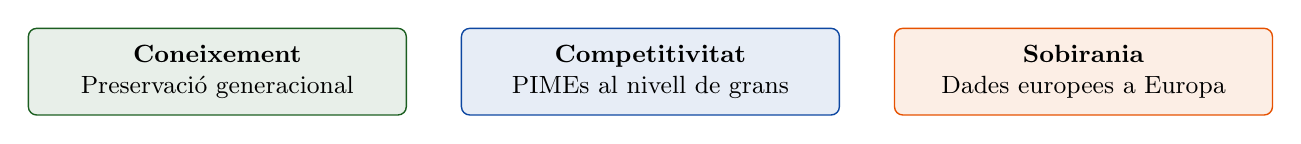
\begin{tikzpicture}[
  box/.style={rectangle, rounded corners=3pt, draw=#1, fill=#1!10,
    minimum width=4.8cm, minimum height=1.1cm, align=center,
    font=\small, line width=0.5pt}
]
\node[box=impactgreen] (a) at (0,0) {\textbf{Coneixement}\\Preservació generacional};
\node[box=impactblue] (b) at (5.5,0) {\textbf{Competitivitat}\\PIMEs al nivell de grans};
\node[box=impactorange] (c) at (11,0) {\textbf{Sobirania}\\Dades europees a Europa};
\end{tikzpicture}
\end{center}

\vspace{0.3em}
\begin{center}
\small\textcolor{midgray}{XC Gradient $\cdot$ Declaració d'Impacte $\cdot$ Confidencial $\cdot$ Abril 2026}
\end{center}

\end{document}
